\chapter{Channel Codes of Seismograms}\label{cha:channel-codes}

Seismic networks, such as the Global Seismographic Network (GSN),
generally involve various types of instruments with different bandwidths,
sampling properties and component configurations. There are standards
to name channel codes depending on instrument properties. IRIS (\url{http://www.iris.edu})
uses SEED format for channel codes, which are represented by three
letters, such as \texttt{LHN}, \texttt{BHZ}, etc. In older versions
of the SPECFEM3D Cartesian package, a common format was used for the
channel codes of all seismograms, which was \texttt{BHE/BHN/BHZ} for
three components. To avoid confusion when comparison are made to observed
data, we are now using the FDSN convention (\url{http://www.fdsn.org/})
for SEM seismograms. In the following, we give a brief explanation
of the FDSN convention used by IRIS, and how it is adopted in SEM
seismograms. Please visit \url{http://www.iris.edu/manuals/SEED_appA.htm}
for further information.\\


\noindent \texttt{\textbf{Band code:}} The first letter in the channel
code denotes the band code of seismograms, which depends on the response
band and the sampling rate of instruments. The list of band codes
used by IRIS is shown in Figure \ref{fig:IRIS_band_codes}. The sampling
rate of SEM synthetics is controlled by the resolution of simulations
rather than instrument properties. However, for consistency, we follow
the FDSN convention for SEM seismograms governed by their sampling
rate. For SEM synthetics, we consider band codes for which $dt\leq1$
s. IRIS also considers the response band of instruments. For instance,
short-period and broad-band seismograms with the same sampling rate
correspond to different band codes, such as S and B, respectively.
In such cases, we consider SEM seismograms as broad band, ignoring
the corner period ($\geq10$ s) of the response band of instruments
(note that at these resolutions, the minimum period in the SEM synthetics
will be less than $10$ s). Accordingly, when you run a simulation
the band code will be chosen depending on the resolution of the synthetics,
and channel codes of SEM seismograms will start with either \texttt{L},
\texttt{M}, \texttt{B}, \texttt{H}, \texttt{C} or \texttt{F}, shown
by red color in the figure.\\


\begin{figure}[ht]
\noindent \begin{centering}
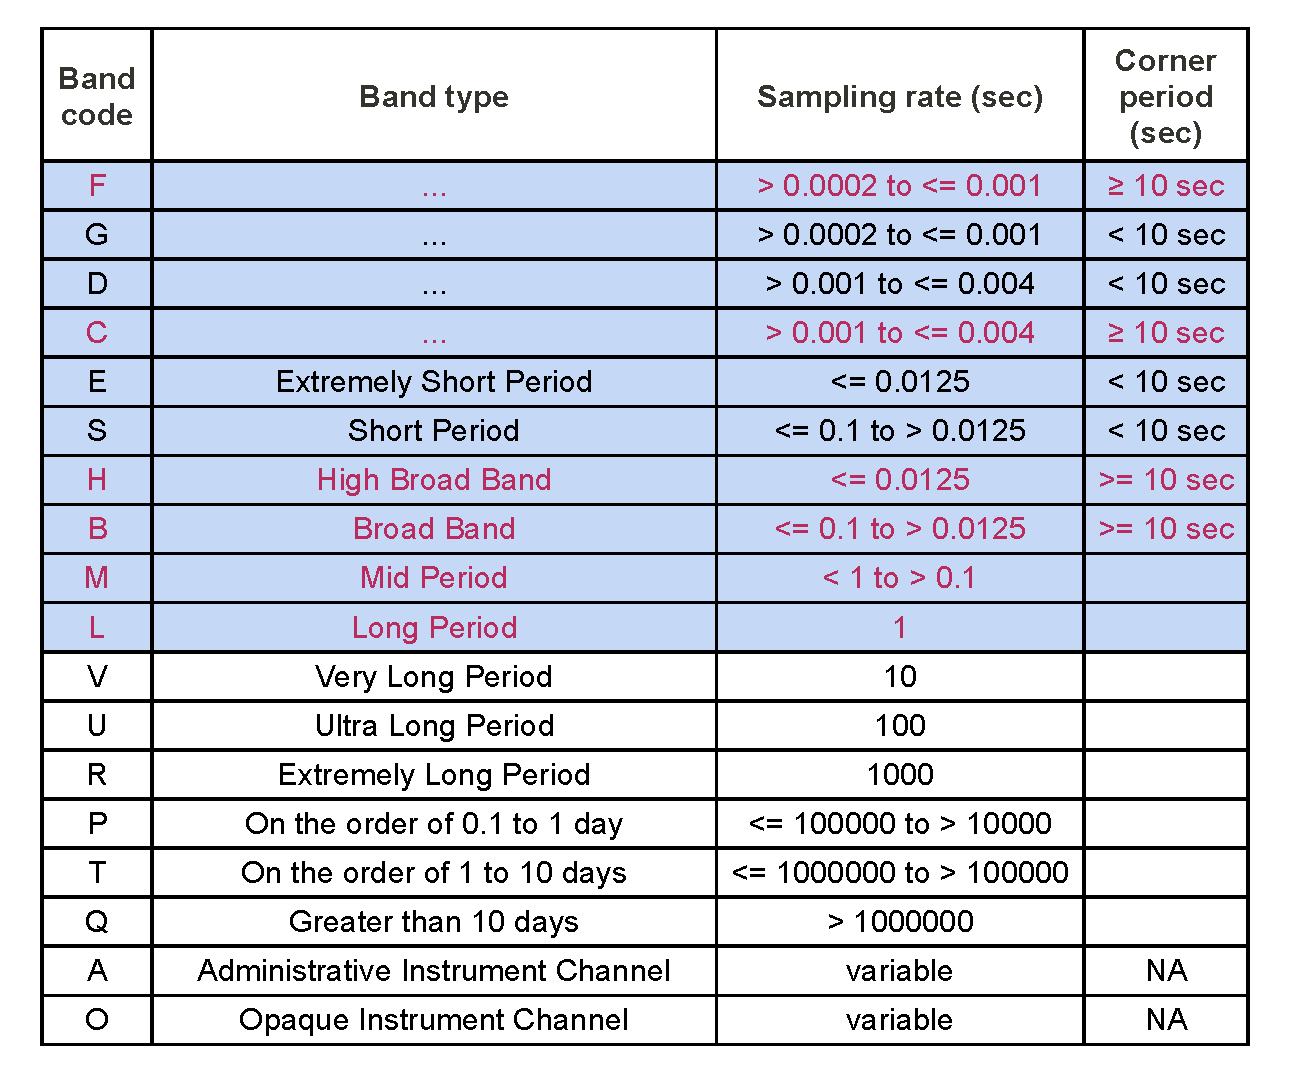
\includegraphics[scale=0.6]{figures/IRIS_band_codes.pdf}
\par\end{centering}

\caption{The band code convention is based on the sampling rate and the response
band of instruments. Please visit \url{http://www.iris.edu/manuals/SEED_appA.htm}
for further information. Grey rows show the relative band-code range
in SPECFEM3D Cartesian, and the band codes used to name SEM seismograms
are denoted in red.}


\label{fig:IRIS_band_codes}
\end{figure}


\noindent \texttt{\textbf{Instrument code:}} The second letter in
the channel code corresponds to instrument codes, which specify the
family to which the sensor belongs. For instance, \texttt{H} and \texttt{L}
are used for high-gain and low-gain seismometers, respectively. The
instrument code of SEM seismograms will always be \texttt{X}, as assigned
by FDSN for synthetic seismograms. \\


\noindent \texttt{\textbf{Orientation code:}} The third letter in
channel codes is an orientation code, which generally describes the
physical configuration of the components of instrument packages. SPECFEM3D
Cartesian uses the traditional orientation code \texttt{E/N/Z} (East-West,
North-South, Vertical) for three components when a UTM projection
is used. If the UTM conversion is suppressed, i.e. the flag \texttt{SUPPRESS\_UTM\_PROJECTION}
is set to \texttt{.true.}, then the three components are labelled
\texttt{X/Y/Z} according to the Cartesian reference frame. \\


\noindent \texttt{\textbf{EXAMPLE:}} The sampling rate is given by
\texttt{DT} in the main parameter file \texttt{Par\_file} located
in the \texttt{DATA/} subdirectory. Depending on the resolution of
your simulations, if you choose a sampling rate greater than $0.01$
s and less than $1$ s, a seismogram recording displacements on the
vertical component of a station \texttt{ASBS} (network \texttt{AZ})
will be named \texttt{AZ.ASBS.MXZ.semd.sac}, whereas it will be \texttt{AZ.ASBS.BXZ.semd.sac},
if the sampling rate is greater than 0.0125 and less equal to 0.1
s.


